\chapter{\oneedge{}: Application orchestration over geo-distributed Edge infrastructure}
\label{sec:oneedge}

\section{Introduction}

\section{Basics of Application Orchestration in Edge Computing}

In this section, we will set the stage for the discussion of how \oneedge{} leverages the mechanisms proposed in this dissertation to implement control-plane policies for application orchestration. We first present the application model that \oneedge{} supports, the application requirements for which control-plane policies need to be designed, and the challenges faced by in an Edge setting due to the dynamism in workload.

\subsection{Application Model}
\label{sec:oneedge_app_model}
Situation-awareness applications process data incoming from sensors through a series of functions, each extracting out certain information from the input data or performing a certain operation. This can be naturally modeled as a Data Flow Graph (DFG) \cite{dfg}. Each node in a DFG represents a processing function and each directed edge represents a data dependency between the upstream and downstream node. In \oneedge{}, we assume a special case of the more general DFG model, which is a pipeline of functions. As shown in \cref{fig:app_pipeline}, each DFG node, or application component, is an independent actor, and is represented by a level. Level 0 is assigned to the most downstream component, and the level number increases as we go upstream toward the client. Each component reads from a queue of input events which is populated by the upstream component and sends output events to the downstream component. An application component is also able to send events to an upstream component (including the client).

\begin{figure}[ht]
\centering
\begin{subfigure}{.48\columnwidth}
  \centering
    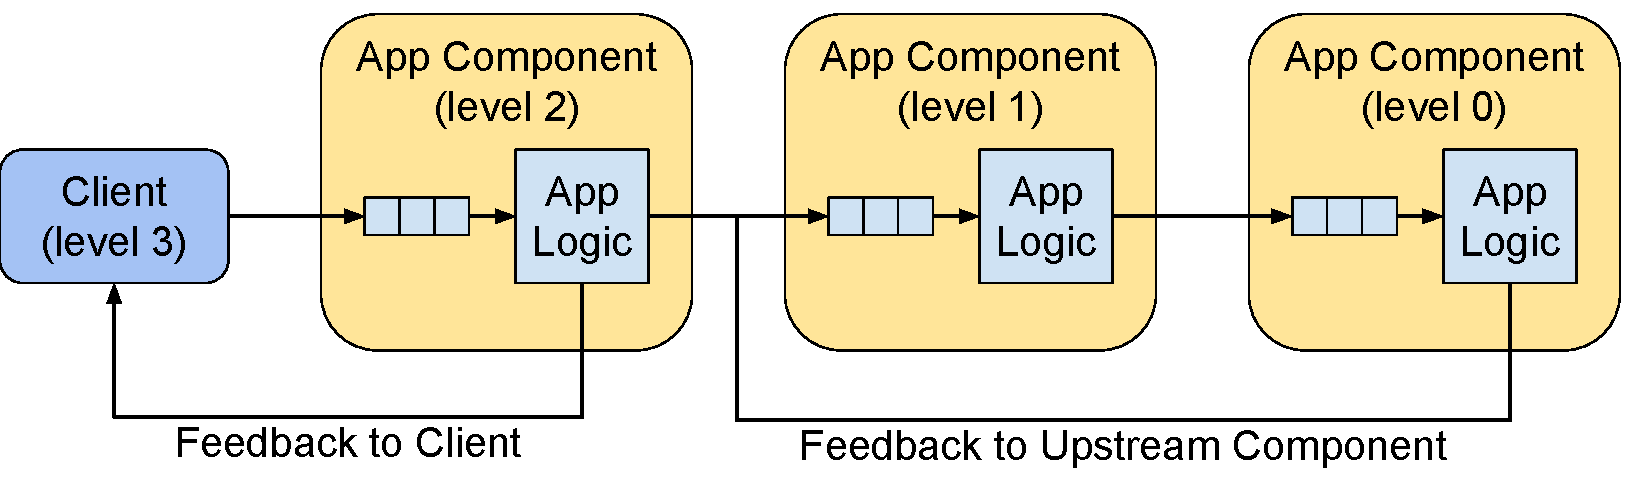
\includegraphics[width=\columnwidth]{figures/oneedge/app_pipeline.pdf}
    \caption{Application Pipeline.}
    \label{fig:app_pipeline}
\end{subfigure}
\begin{subfigure}{.48\columnwidth}
  \centering
    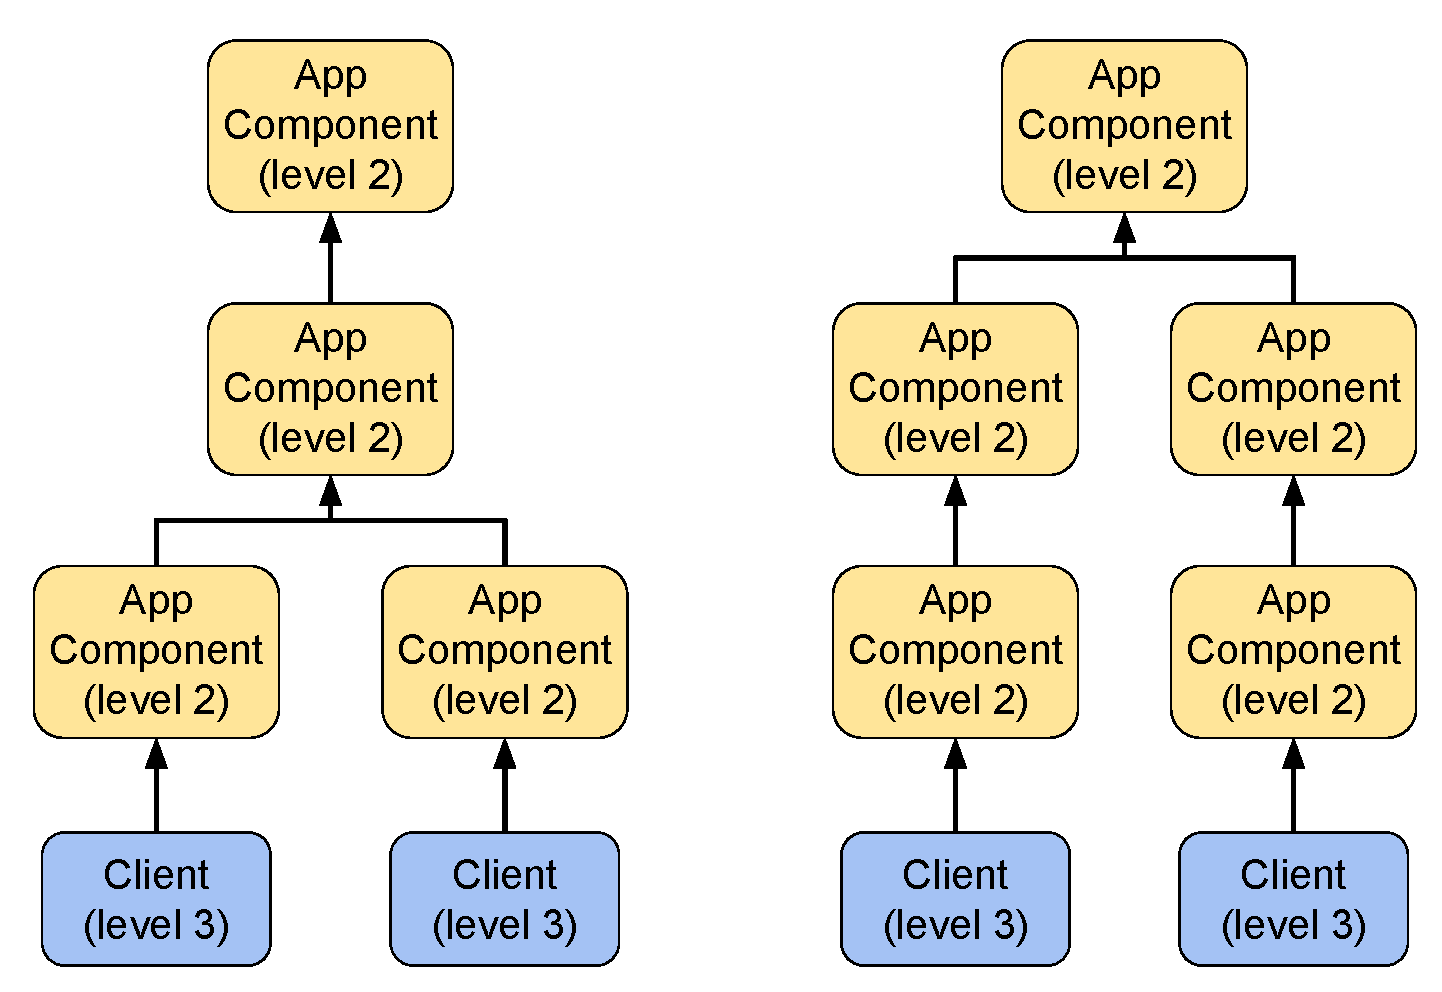
\includegraphics[width=\columnwidth]{figures/oneedge/pipeline_tree.pdf}
    \caption{Actual deployment of a pipeline-based application model resembles a forest with multiple trees.}
    \label{fig:pipeline_tree}
\end{subfigure}
\caption{Description of the application model.}
\label{fig:app_model}
\end{figure}

Although applications are modeled and specified as a linear pipeline, upon deployment for multiple clients, world, the set of application components and the data dependencies among them resemble a forest, as shown in \cref{fig:pipeline_tree}. This is because in order to serve many geo-distributed clients, the same application component needs to have several instances deployed in network proximity of clients so that communication latency to the application instance can be minimized and real-time response made possible. However, not all pipeline components have stringent latency requirements, and thus can serve multiple clients. Each tree in the forest has the most downstream application component (with level 0) as the root node and clients as leaf nodes. Each root-to-leaf path in a tree is a complete application pipeline, and we call each such path except the leaf node an \textit{application instance}. An application component that serves more than one upstream components is essentially processing information gathered from multiple clients, and therefore is able to enable state sharing among clients. However, even for applications that don't share state among clients in their logic, sharing one or more components in the application pipeline among multiple clients can be beneficial. This is because the memory footprint of running multiple independent application components is higher than sharing an application component to serve the same number of clients \todo{quantify?}.

\begin{figure}[ht]
\centering
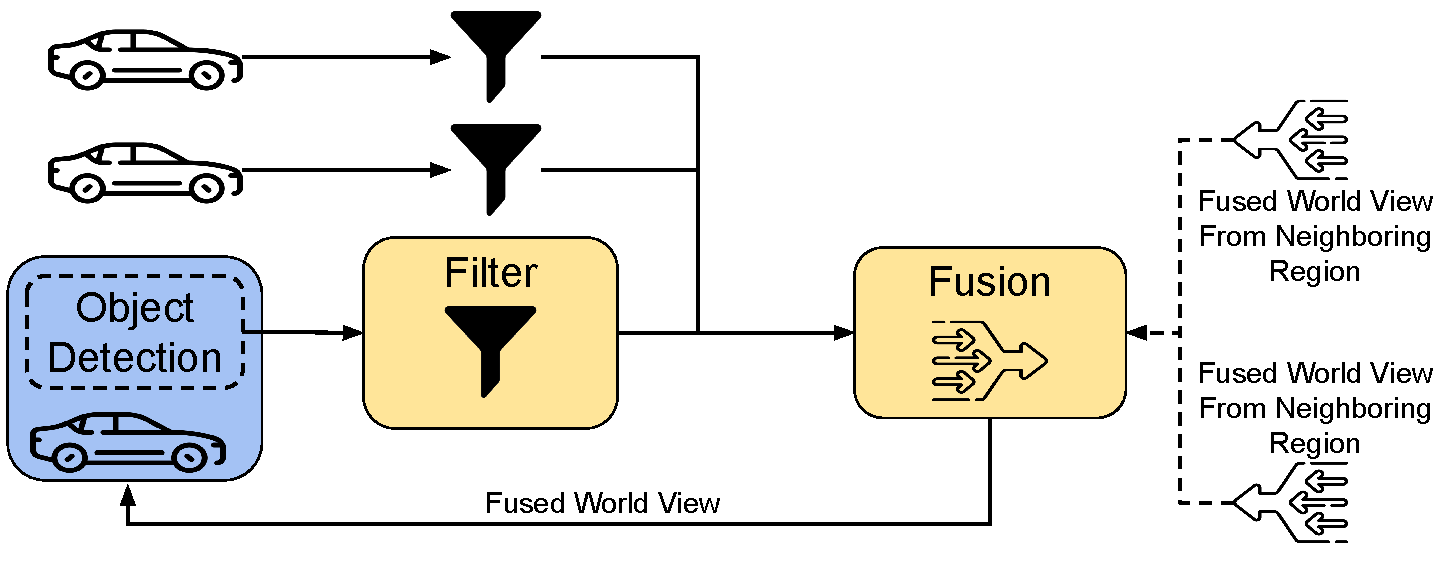
\includegraphics[width=0.8\columnwidth]{figures/oneedge/collaborative_driving_app.pdf}
\caption{The collaborative driving assistance application modeled as a pipeline of components.}
\label{fig:collab_driving_pipeline}
\end{figure}

\par For example, the Collaborative Driving Assistance application can be modeled as a pipeline of application components as shown in \cref{fig:collab_driving_pipeline}. The Client component performs object detection on an input LiDAR sensor stream to generate a list of objects that it can see in its immediate field of view. The Sub-Regional View component aggregates the individual views from multiple vehicles that are in close spatial proximity of one another to create a composite view. This composite view is fed back to the vehicles so that they can improve their lane control and collision avoidance decisions. The output of Sub-Regional View components is processed by the Regional View component to perform higher-level analyses across a larger geographical area.

\begin{comment}
\subsubsection{Programming Model}
\begin{table}
\caption{Programming model API:  communication primitives.}
\label{table:comm_api}
\centering
\resizebox{0.95\textwidth}{!}{%
\begin{tabular}{|c|c|}
\hline
\textbf{Interface} & \textbf{Description} \\ \hline
\begin{tabular}{@{}c@{}} void send\_up (message m, edgeId o) \end{tabular} & \begin{tabular}{@{}c@{}} Sends a message asynchronously from a node \\ to the downstream node connected through edge \textit{o}. \end{tabular} \\ \hline
\begin{tabular}{@{}c@{}} void send\_down (message m, edgeId i,\\ \textbf{optional } nodeId n) \end{tabular} & \begin{tabular}{@{}c@{}}Sends a message asynchronously to all upstream \\nodes connected through edge \textit{i}.  Optionally it can \\ choose to only contact  one of the upstream nodes \textit{n}. \end{tabular} \\ \hline
\begin{tabular}{@{}c@{}} void send\_to (message m, \\nodeId destination) \end{tabular} & \begin{tabular}{@{}c@{}}Sends a message to a specific destination node.
\end{tabular} \\ \hline
\begin{tabular}{@{}c@{}} void send\_to\_partion\_clients (message m, \\partitionId id) \end{tabular} & \begin{tabular}{@{}c@{}}Sends a message to all the clients in a logical partition.
\end{tabular} \\ \hline
\end{tabular}
}
\end{table}
\end{comment}

\subsection{Decisions taken by an Application Orchestrator}
\label{sec:app_orch_decisions}
Effective orchestration of situation-awareness applications on Edge infrastructure requires two main decisions that need to be taken by the control-plane. These two decisions are (i) mapping clients to application instances, and (ii) deploying and managing resources for application instances on Edge sites.

\subsubsection{Mapping Clients to Application Instances}
\newcommand{\clientset}{\mathcal{C}}
\newcommand{\instanceset}{\mathcal{I}}
\newcommand{\resourceset}{\mathcal{R}}

We now formally describe the decision concerning mapping clients to application instances for a specific application. Let $\clientset$ denote the set of clients for the given application and $\instanceset$ denote the set of running instances of all the components of this application. As mentioned before, each application component in $\instanceset$ as well as each client in $\clientset$ has an associated level, which indicates the stage number in the pipelined application model. The mapping of clients and upstream application components to downstream components is defined by a function $\mathcal{M}$, defined in \cref{eq:mapping_domains_eqns} and \cref{eq:mapping_eqn}.
\begin{equation}
\label{eq:mapping_domains_eqns}
\mathcal{M} : \left( \clientset \cup \instanceset \right) \times Z^+ \rightarrow \instanceset
\end{equation}

\begin{equation}
\label{eq:mapping_eqn}
\mathcal{M} \left( c, l \right) = \text{App Component of level }l \text{ serving }c
\end{equation}
The control-plane needs to compute such a mapping so as the ensure that the application requirements discussed in \cref{sec:oneedge_app_reqs} are satisfied.

\subsubsection{Deployment of Application Instances on Edge Sites}
Each application instance, comprising of all the components in the application's pipelined model, need to be deployed on a compute resource. The placement of application components ($\instanceset$) on the set of compute resources ($\resourceset$) can be represented by the function $\mathcal{P}$, as described in \cref{eq:placement_domain_eqn} and \cref{eq:placement_eqn}.

\begin{equation}
\label{eq:placement_domain_eqn}
\mathcal{P} : \instanceset \rightarrow \resourceset
\end{equation}

\begin{equation}
\label{eq:placement_eqn}
\mathcal{P} \left( a \right) = \text{Compute resource hosting }a
\end{equation}
The placement of application components is computed in a manner that meets the end-to-end latency requirements of the application, as described in \label{sec:oneedge_app_reqs}.

\subsection{Application Requirements}
\label{sec:oneedge_app_reqs}
We now discuss the requirements that \oneedge{} allows application developers to specify which allow the application
\begin{figure}
	\centering
	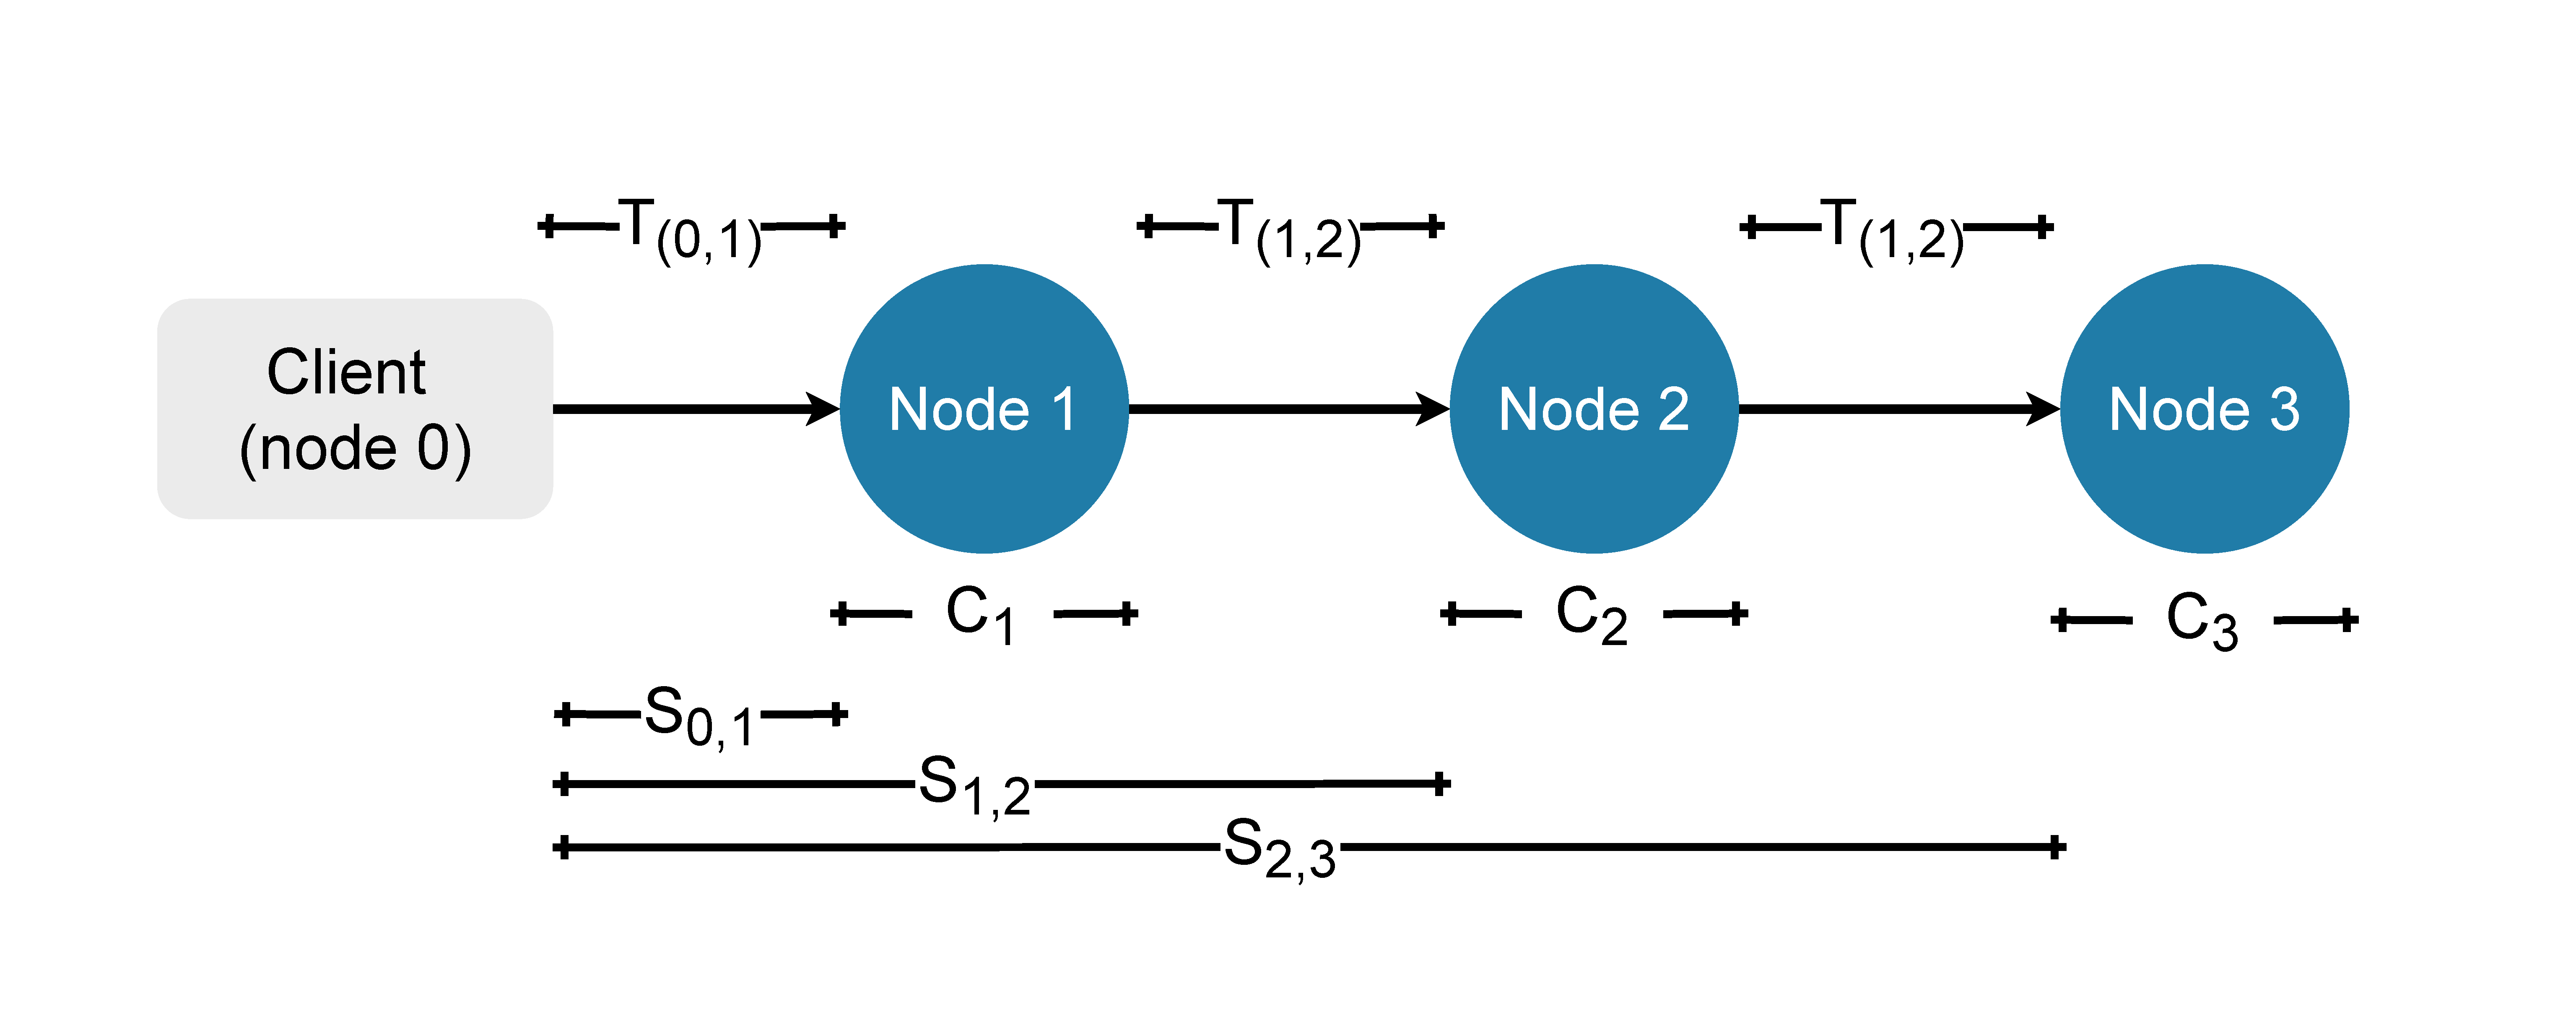
\includegraphics[width=0.95\textwidth]{figures/oneedge/pipeline_latency.pdf}
    \caption{
    A generic pipeline that explains the different components of the tolerable latency staleness. $S_{(i-1,i)}$ is the acceptable latency starting at the output of the client to the input of the node $i$. It is composed of both computational latency $C_j$ and transmission latency $T_{j-1,j}$.}
	\label{fig:pipeline_lat}
\end{figure}

\subsubsection{End-to-End Processing Latency}
Application developers are able to specify the end-to-end processing latency for each component in the application pipeline model. End-to-End processing latency for an application component is the time elapsed between when a specific data-item/event is generated by the client to when it is processed by the application component. This includes the network transmission latency and processing time of all the upstream components. The end-to-end latency constraint for each application component should be satisfied for each client of the given application. The end-to-end latency for client $c$ at application component with level $l$ is defined in \cref{eq:e2e_proc_latency}, which is calculated recursively using the value for the upstream component with level $l+1$. The base case is when the level $l$ equals the level corresponding to the client itself, in which case, the end-to-end latency is equal to the processing latency on the client.
\begin{equation}
\label{eq:e2e_proc_latency}
E2E \left( c, l \right) = E2E \left(c , l+1 \right) + proc \left( \mathcal{M} \left( c, l \right) \right) + net \left(  \mathcal{M} \left( c, l+1 \right) , \mathcal{M} \left( c, l \right) \right)
\end{equation}

\subsubsection{Spatial Affinity}
Several situation-awareness applications such as the collaborative driving assistance application (\cref{fig:collab_driving_pipeline}) consist of components that are tied to a specific geographical area, and are meant to serve clients located in that geographical area only. This is meant to enable information sharing between clients that are in close spatial proximity to one another. We denote the geographical area served by an application component as its \textit{spatial context}. The partitioning of the geographical space into spatial contexts is application-specific. More precisely, the application developer would specify a function $\mathcal{S}$ that maps a geographical location $\left( x , y \right)$ to a unique spatial context $s_z$ (identified by a positive integer $z$) (\cref{eq:spatial_context}).

\begin{equation}
\label{eq:spatial_context}
   \mathcal{S}: X \times Y \rightarrow \{ s_0, s_1, \cdots \}
\end{equation}
\begin{equation}
   X = \{x \in \mathbb{R}~|~-\pi < x < \pi\}
\end{equation}
\begin{equation}
   Y = \{y \in \mathbb{R}~|~\dfrac{-\pi}{2} < y < \dfrac{\pi}{2}\}
\end{equation}

For an application component of level $l$ that needs to facilitate inter-client information sharing, the control-plane assigns each spatial context $s_z$ with an application component and map all clients located within that spatial context to that instance. Multiple spatial contexts can also be mapped to the same application instance. However, the main requirement is that all clients within given spatial context should be served by the same application instance so that they can effectively share state with other clients in the same spatial context. The quality of this client-application-instance mapping is quantified using the Spatial Alignment metric, as shown in \cref{eq:spatial_alignment}. The Spatial Alignment metric is defined for each spatial context $s_z$ that is served by the application component instance $a$ at level $l$.  Ideally, the spatial alignment metric should be equal to 1 for all spatial contexts.
\begin{equation}
\label{eq:spatial_alignment}
SA \left( a \right) = \dfrac{|\{ c \in \clientset : c.loc \in s_z   \mathcal{M} \left( c, l\right) = a \}|}{|\{ c \in \clientset : c.loc \in s_z \}|}
\end{equation}
\todo{Can we connect application instance $a$ with $s_z$?}

\subsection{Application Abstract: Specifications provided by the Developer}
\oneedge{} expects the developer to provide specifications for each application, which should contain information that will be used by the control-plane for making policy decisions. The application abstract should contain the number of levels in the application pipeline, the expected inter-arrival time of sensor data at each client and the following fields for each level of the pipeline.
\begin{itemize}
\item The end-to-end latency constraint for that level. This information is used by the application scheduling policy in the control-plane to ensure that the end-to-end latency observed by all workers that belong to this particular application and level satisfied this constraint. This information is also used by the violation detection policy to detect a violation in end-to-end latency and trigger a reconfiguration.
\item The number of CPU cores and memory (in KB) required by a worker of that level. These are denoted by $CPU_{req}$ and $MEM_{req}$ respectively.
\item The expected processing latency of the worker for different number of clients connected to it. This information is obtained by offline-profiling of the application component by the developer. This information is used by the application scheduling policy to estimate the processing latency of a worker.
\item Maximum number of clients that can be connected to a worker of that level. This information is obtained by offline profiling of the application component and determining when the worker cannot handle any more clients without a significant increase in processing latency. This information is used by the application scheduling policy to select candidate workers for reuse.
\end{itemize}

\subsection{Challenges in Achieving Application Objectives}

\subsubsection{Heterogeneity in Edge Infrastructure Topology}
\begin{itemize}
\item Network connectivity between Edge Sites that belong to the same geographical area is heterogeneous.
\item Communication latencies between Edge Sites and between clients and Edge Sites depends on how the Edge Sites and clients connect to the network and the peering between the different providers serving these entities.
\item For a particular instance of an application, not all Edge Sites are equally suitable for hosting the different application components.
\end{itemize}

\subsubsection{Client Mobility}
Typical situation-awareness applications have clients that are inherently mobile, for example, vehicles, pedestrians, UAVs, etc. The mobility of clients creates two main challenges. For applications involving inter-client information sharing, the mapping of a client to an instance of a given component is based on the spatial context of that component's instance and the location of the client. Due to client mobility, the client's location might change so much that it exits the spatial context of the current application component instance, and thus is not able to coordinate with the correct subset of other clients that are in its physical proximity. This requires that the client be migrated to the application component instance that has the correct spatial context which corresponds to the current location of the client. Secondly, client mobility can result in a change in the network routing and hence communication latency to and from the application instance. This change in communication latency affects the end-to-end processing latency for that client's data by the current application instance. This necessitates that the client be migrated to an application instance that can satisfy the end-to-end latency requirements.

\subsubsection{Changes in Processing Requirements of Applications}
The frequency of events generated by different application components in an application pipeline changes over time. This is either due to the mobility of clients which changes the properties of the environment sensed by the clients. For instance, in the Collaborative Driving Assistance application, the number of neighboring vehicles output by the Detection component (in the client) is a function of the density of neighboring traffic, which changes with time as the ego vehicle moves. The change in processing requirements of applications can also happen for static sensors, such as CCTV cameras, when the environment they are sensing undergoes changes. For instance, in the \todo{} application, the frequency of events generated by the \todo{} component depends on the number of cars in the field-of-view of a camera, which changes over time.

\subsection{Edge-centric Policies for Application Orchestration}
\begin{itemize}
\item Application Placement that takes into account end-to-end latency threshold of application components as well as spatial affinity requirement.
\item Continuous monitoring of application instances to detect violation of end-to-end processing latency or spatial affinity requirements.
\item In the case of a violation, a root-cause analysis needs to be done to detect the root-cause of the violation and trigger an appropriate reconfiguration action.
\item The reconfiguration action depends on the nature of the violation. If the violation is due to communication latency increase between an upstream and downstream component, the downstream component instance needs to be mapped to a different instance of the upstream instance so that the latency requirements can be satisfied. If the violation is due to compute overload, a portion of the clients served by the overloaded instance need to be migration to a different application instance. If the overloaded instance is spatially constrained, then the partitioning of clients has to be done so as to ensure that the resulting mapping of clients satisfies spatial affinity requirements.
\end{itemize}

\section{Architectural Components of \oneedge{}}
Now we present the system architecture of \oneedge{}, covering the design choices and deployment characteristics of each component of the system. We will first provide a high-level overview of the system, with an emphasis on describing how \oneedge{} operates and the typical operations of each component. Then we will discuss the functions of each component in more detail.

\subsection{High-level System Architecture}
\begin{figure*}[t]
\centering
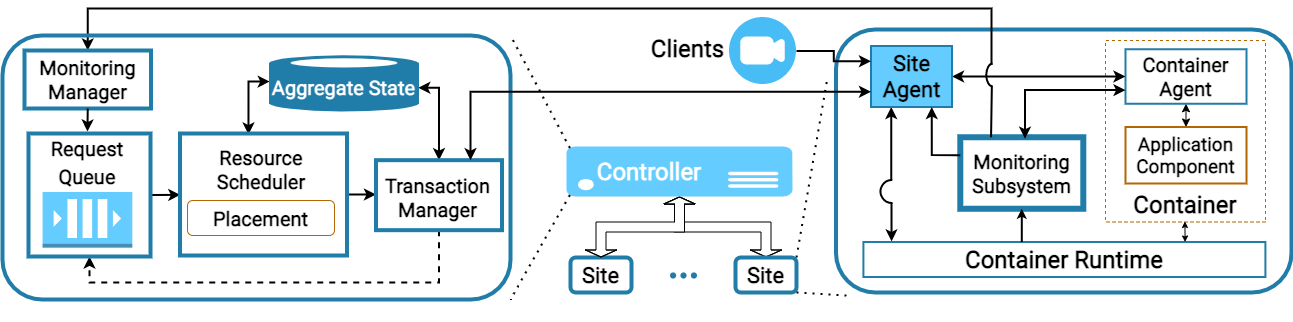
\includegraphics[width=0.85\columnwidth]{figures/oneedge/onefog_overview.png}
\caption{\oneedge{}'s System Architecture. A central controller (left blow-up) coordinates with all the Edge sites (right blow-up).}
\label{fig:system_arch}
\vspace{-2mm}
\end{figure*}
\cref{fig:system_arch} shows the high-level system architecture of \oneedge{}. There are three top-level entities \textit{Clients}, \textit{Edge Sites} and the \textit{Controller}. 
Client entities represent all client devices, such as autonomous vehicles, drones, etc. that run the client component of situation-awareness applications. Clients entities are inherently mobile and geo-distributed. The client module of situation-awareness applications hosted by them require connection to an application pipeline that can carry out the rest of the functionality of the application. Each client is also equipped with sensor and actuator devices. Sensors on the client act as the source of data for the application pipeline. 
\par Edge Sites geo-distributed entities with compute and storage resources that is able to run instances of application components and serve clients. The Controller is a logically-centralized entity which is responsible for performing the main decisions of an application orchestrator, i.e., mapping upstream application workers to downstream workers, and deploying and managing workers (\cref{sec:app_orch_decisions})\todo{Define workers before}. It does so by maintaining the state of the entire infrastructure, including clients, edge sites and the workers running on edge sites. The controller receives requests from clients for connection to an application pipeline and it uses the application scheduling policies against the aggregate state to make this decision. In addition, the controller also hosts the policies for detecting violation of application requirements and triggering reconfiguration actions by invoking the aforementioned application scheduling policies.

\subsection{Client}
In the \oneeedge{} application orchestration system, a Client consists of three key components - the Client Worker that hosts the client application module, Worker Agent which acts as the interface between the application module and the rest of the system and the Sensor and Actuator devices, which are the source and sink of data.

\subsubsection{Client Worker}
The Client Worker hosts the application logic of the given application that needs to run on client devices. It is responsible for communication with the sensor and actuator devices present on the client. The Client Worker processes data from the sensor and sends the extracted information to the downstream application component. The Client Worker also receives information from the downstream component which it processes to generate commands for the actuator devices.

\subsubsection{Client Worker Agent}
The Client Worker Agent is an instance of \oneedge{}'s Worker Agent, which acts as the interface between the application logic and the rest of the system. Firstly, the worker agent calls the \textit{on\_message\_arrival} handler in the client worker whenever a message is received from the sensor. Second, the worker agent is responsible for communicating with the controller to establish a connection with a downstream application component. When the client worker generates a message that needs to be sent to the downstream worker, the worker agent is responsible for sending it to the worker agent of the downstream worker, which then passes it to the corresponding worker. Furthermore, it also serves as a part of the monitoring subsystem, whereby it collects metrics related to the execution of the client worker and forwards them for further processing.

\subsection{Site}
An Edge site consists of four main components, as shown in the right blow-up in \cref{fig:system_arch} - the Site Agent, Container Runtime, Worker Agent and the Monitoring Subsystem. 
\subsubsection{Site Agent}
The Site Agent component is responsible for managing the resources on the site, along with the application component instances running on the site. It interfaces with the central Controller for the scheduling of applications on that Edge site. The Site Agent is responsible for launching application component instances on the Edge Site and allocating resources to those instances.

\subsubsection{Container Runtime}
The Container Runtime is the software platform upon which the various application component instances run as containers. The container runtime provides primitives for launching containers based on an application-specific image, allocation a specific amount of compute and memory resources to containers to ensure predictable performance and isolation, access to a filesystem for storing ephemeral state and communication with other entities in the system. 

\subsubsection{Worker Agent}
The Worker Agent is a software agent which is deployed alongside the application logic within each application component instance's container. It acts as the interface of the application logic for that specific application component with the rest of the components and the outside world. It does so by implementing the various interfaces provided to the application developer. The worker agent facilitates communication between various application instances by allowing upstream and downstream components to send messages to each other, as well as trigger callback functions in the application logic upon message arrival. Furthermore, it also serves as a part of the monitoring subsystem, whereby it collects metrics related to the execution of the application component and forwards them for further processing.
\subsubsection{Monitoring Subsystem}
\todo{Add text for the Monitoring Subsystem.}

\subsection{Controller}
The Controller is responsible for application scheduling and management at a global-scale across Edge sites. It receives requests for application deployment and reconfiguration from clients and the monitoring subsystem respectively. These requests are processed by the Scheduler, which turns these requests into a transaction (set of actions) to be executed on one or more Edge sites. The transactions are executed on the Edge sites by the Transaction Executor component. We will discuss each of the components in greater detail next.
\subsubsection{Scheduler}
\label{sec:scheduler}
The Scheduler picks up one request at a time from the Controller's request queue and computes a scheduling decision for the request. The scheduling decision is computed by executing the placement algorithm (\cref{todo}) for mapping the requesting client to a suitable application instance that can satisfy the end-to-end latency and spatial affinity requirements. If no such application instance exists, a new instance is instantiated and suitable Edge sites for hosting the application components are selected. In the case of a reconfiguration request for updating allocation of an application instance, the scheduler computes the final resource allocation for the components of that application instance.
\par The Scheduler reads the Aggregate Resource State to check the current available resource capacity on each Edge site, and updates the state with changes to the resource allocation. Hence, the Aggregate State is \textit{optimistically} updated even before the scheduling decision has actually been applied on the specific Edge sites. By doing so, the process of compute application scheduling decisions is decoupled from the actual enforcement of those decisions on the Edge sites. The scheduling decision is in the form of a Transaction, which is a collection of the actions that need to be taken to execute the scheduling decision. The constituent actions of a transaction need to executed on one or more Edge sites. 

\begin{comment}
\begin{minted}{yaml}
-   app_id: 
    txn_id: 
    actions: 
        -   site_id: 
            site_actions:
                -   level: 
                    type: DEPLOY
                    resources: 
                        cpu:
                        memory: 
                -   level: 
                    type: MODIFY_ALLOC
                    resources:
                        cpu: 
                        memory:
\end{minted}
\end{comment}

\subsubsection{Aggregate State}
\label{sec:aggr_state}
The Aggregate State contains information about the Edge Sites, application clients and workers, which is used by the application scheduling policy for making decisions. The Aggregate State contains the following data structures.
\begin{itemize}
\item \textit{\textbf{sites}}. The Aggregate State maintains a dictionary containing all the Edge Sites' information. They key of the dictionary is the ID of an edge site, while the value is an $EdgeSiteMetadata$ data structure which contains the following fields.
\begin{itemize}
\item The total CPU and memory capacity of the edge site $CPU_{total}, MEM_{total}$. $CPU_{total}$ is expressed in number of CPU cores, while $MEM_{total}$ is expressed in kilobytes (KB).
\item The network coordinate of the edge site, denoted by $NC_{site\_id}$.
\end{itemize}
\item \textit{\textbf{clients}}. The Aggregate State maintains a dictionary containing information of all the clients present in the system. The $clients$ dictionary maps the ID of a client to an instance of the $ClientMetadata$ data structure, which contains the following fields.
\begin{itemize}
\item The application ID of the client, denoted by $app\_id$.
\item The network coordinate of the client, denoted by $NC_{client\_id}$.
\end{itemize}
\item \textit{\textbf{workers}}. The Aggregate State maintains information about the application workers currently hosted on edge sites in the $workers$ dictionary. The key of the $workers$ dictionary is ID of an edge site, and the value is a lower-level dictionary specific to that edge site. The lower-level dictionary maps the ID of a worker to an instance of the $WorkerMetadata$ data structure, which contains the following fields describing a particular worker.
\begin{itemize}
\item The ID of the edge site on which the worker is hosted, denoted by $site\_id$.
\item The number of CPU cores and memory (in KB) allocated to the worker, denoted by $CPU_{alloc}$ and $MEM_{alloc}$ respectively.
\item The application ID and level of the worker, denoted by $app\_id$ and $level$ respectively.
\item The number of clients connected to this application worker, denoted by $curr\_clients$.
\end{itemize}
\item \textit{\textbf{parent\_map}}. As discussed in \cref{sec:oneedge_app_model}, clients and application workers have a parent-child relationship, wherein the parent worker for a child client or worker represents the downstream worker which receives output data from the child client or worker. A worker can have one or more children, but at most one parent. The aggregate state stores this parent child relationship in the form of a dictionary, which maps the ID of the child worker or client to the ID of the parent worker and the ID of the site on which the parent worker is hosted.
\end{itemize}
As described in \cref{sec:scheduler}, the Aggregate State is used by the Scheduler to make application scheduling decisions. For subsequent requests' processing to be aware of the decisions made for the current request, the Aggregate State is updated with the current request's decisions. 

\begin{comment}
\begin{itemize}
\item The Aggregate State maintains an optimistic version of the resource allocation state, assuming that all the scheduling decisions taken by the Scheduler will successfully get enforced on the Edge sites.
\item However, since Site Agents have the autonomy to make resource allocation changes without coordinating with the Controller, scheduling decisions from the Controller could be rejected by the Site Agent, in which case the corresponding Transaction would be aborted.
\item The abortion of a transaction would result in rolling back the Aggregate State to a state before the aborted transaction's processing was begun by the Scheduler.
\item In addition to having applied updates that have not yet been successfully applied on Edge sites, the Aggregate State is also eventually consistent with the ground-truth resource allocation which is maintained by the Site Agents. Since Site Agents are able to update allocation state of the site without coordinating with the Controller, the Controller's Aggregate State does not see those autonomous updates until the state is synchronized with the Edge site, which is done periodically.
\end{itemize}
\end{comment}

\begin{comment}
\subsubsection{Pending Transactions Pool}
The Transactions generated by the Scheduler are buffered in the Pending Transactions Pool so that their constituent actions can be enforced on the Edge sites. However, transactions can only be executed in the order in which they were processed by the Scheduler. The relationship between transactions that defines the order in which they are executed can be denoted as $T_i \leftarrow T_j$, in this case denoting that the transaction $T_i$ can be executed only when $T_j$ is executed. In other words, the Aggregate State output by $T_j$ was used as input for $T_i$. The following conditions have to be met for $T_i \leftarrow T_j$ to be true:
\begin{itemize}
\item $T_j$ was generated by the Scheduler before $T_i$.
\item The set of Edge sites affected by $T_i$ and $T_j$ overlap.
\end{itemize}
\end{comment}

\subsubsection{Transaction Executor}
The Transaction Executor module is responsible for executing the decisions taken by the Scheduler on the Edge Sites. It sends commands for instantiating workers and allocating resources to them on the target Edge sites.

\section{Latency-aware Application Scheduling using Network Proximity Estimation}

\subsection{Deployment of Network Coordinate Agents}
Network Coordinate agents are deployed on all Edge Sites's Site Manager modules, Edge Gateways and Clients. The agents on the clients don't participate in the decentralized network coordinates protocol, but rather compute their own network coordinate by using the coordinate of their current edge gateway. All agents periodically send their current network coordinate to the controller, which maintains them in its aggregate state can be queried by the application scheduling policy.

\subsection{Estimating End-to-End Processing Latency}
\par Estimating the end-to-end latency observed at a worker (instance of an application pipeline stage) is equal to the sum of the processing and communication latencies of all the upstream workers including itself. 
\par Estimating the communication latency is done by using the Network Proximity Estimation mechanism. The network latency between the client and its \textit{parent} worker is computed by using the network coordinate of the client and the network coordinate of the Edge Site hosting the worker. Similarly the network latency between a \textit{parent} and a \textit{child} worker is computed using the network coordinates of the two Edge Sites hosting those workers.
\par The processing latency of a worker is derived from the developer's specification, provided as part of the application abstract. In the context of \oneedge{}, queuing latency at a worker is also included in processing latency. The processing latency of a worker depends on the number of clients it is serving. The developer is expected to perform offline profiling of each application component to generate the distribution of expected processing latencies for a given number of clients served by a worker.

\subsection{Control-Plane Policy for Latency-aware Application Scheduling}
\label{sec:oneedge_latency_aware_placement}
The Latency-aware Application Scheduling policy aims to place applications components on the geo-distributed Edge infrastructure such that end-to-end processing latency requirements of each application component is met as well as scarce Edge resources are used only for latency-sensitive application components. A greedy placement policy would place all components of the application on the Edge, which would result in scarcity of resources to support new clients.
\par \oneedge{}'s latency-sensitive application scheduling policy is illustrated in \cref{algo:oneedge_scheduling_policy}. The algorithm jointly performs the mapping of upstream application workers to downstream ones along with the creating of new workers if they don't exist. The algorithm starts with the client worker, and tries to map it to an existing downstream worker or create a new downstream worker, and so on. This process is executed in the $find\_pipeline$ function, which performs a backtracking search to find the right downstream worker to map the current worker to, assuming that rest of the downstream workers will also find a suitable mapping. In every step of this iterative process, the algorithm maintains the end-to-end processing latency that has been consumed
up to and including the current worker. Line 3 shows that when mapping the client worker to a downstream component, the current cumulative end-to-end latency is assigned a value equal to the processing latency of the client worker. The function $find\_pipeline$ recursively computes the optimal workers for each component of the application pipeline. The result of the $find\_pipeline$ function contains a list of workers for each downstream application component along with information about whether that worker already existed in the system or if it needs to be created (line 7). The metadata of those workers that need to be created is passed to the Transaction Executor module (line 13).

\begin{algorithm}
\caption{Latency-aware Application Scheduling Policy}
\label{algo:oneedge_scheduling_policy}
\begin{algorithmic}[1]
\Require Client c
\Require Aggregate State $\mathcal{A}$
\Require Application Abstract $app\_abstract$

\State $appid \gets app\_abstract.app\_id$
\State $client\_level \gets app\_abstract.num\_levels-1$
\State $cum\_e2e\_latency \gets c.proc\_latency()$ \Comment{End-to-end latency consumed so far}
\State $P \gets find\_pipeline \left( c, client\_level - 1, appid, cum\_e2e\_latency, app\_abstract, null \right)$
\State $W \gets []$ \Comment{Worker launch actions}
\State $child \gets c.id$
\For{$\left( w, create \right) \in P$} \Comment{Establishing parent-child relationship in aggregate state}
    \State $\mathcal{A}.parent\_map[child] \gets \left( w.worker\_id, w.site\_id \right)$
    \State $\mathcal{A}.workers[w.site\_id][w.worker\_id].curr\_clients ++$
    \State $child \gets w.worker\_id$
    \If{$create == True$}
        \State $W += \left( w \right)$  \Comment{If $w$ is a new worker, it is scheduled to be launched}
    \EndIf
\EndFor
\State $launch\_workers \left( W \right)$
\State \Return $P$
\end{algorithmic}
\end{algorithm}

The $find\_pipeline$ function is the central piece of the application scheduling policy. It takes a particular worker as input and the cumulative end-to-end latency up to that worker and tries to find a mapping for the rest of the downstream application components. It does so recursively by trying to map the input worker to an immediately downstream worker, and then calls the function for this downstream worker. If it cannot find a mapping, it backtracks and tries another downstream worker.
\par First, the function tries to reuse existing application workers, since each application component can serve more than one client. It gathers the candidates for worker reuse in line 5 (pseudocode for this function is shown in \cref{algo:get_reuse_candidates}). For each such reuse candidate, if it can serve an additional client (line 7) and if the end-to-end processing latency will be less than the threshold (line 8-9), this candidate is considered, and a recursive call is made to find a mapping for the remaining components. If the recursive call returns a successful result, then the search is complete and the result is returned, along with the chosen worker (lines 11-12).
\par If no reuse candidates work, the policy will need to create a new worker. To do so, it selects the site which should hold this worker such that the latency constraint is satisfied. It computes the maximum network latency that can exist between the current worker and the candidate site in line 15, which is the difference between the latency threshold of the application component to be created and the sum of the total latency spent so far along with the expected processing latency of the application worker to be created. Any edge site within this latency from the current worker can host the downstream worker. The pseudocode of finding candidate sites is presented in \cref{algo:get_candidate_sites}. If the candidate site has enough free resources (line 18) and it can satisfy latency requirements (line 19-20), then a new worker is added on the site in  the aggregate state and a recursive call to the algorithm is made. If the recursive call fails to find a solution, the newly created worker is deleted and the next candidate site is tried.

\begin{algorithm}
\caption{$find\_pipeline$}
\begin{algorithmic}[1]
\Require Child worker/client $child$
\Require Worker level to start search $worker\_level$
\Require Application abstract $app\_abstract$
\Require Cumulative end-to-end latency spent so far $cum\_e2e\_latency$
\Require Worker to select forcefully $force\_worker$
\If{$worker\_level < 0$} \Comment{Search is complete}
    \State \Return []
\EndIf
\State $L \gets app\_abstract.level\_cfgs [worker\_level]$
\State $appid \gets app\_abstract.app\_id$
\State $reuse\_candidates \gets get\_reuse\_candidates \left( appid, worker\_level,  force\_worker \right)$
\For{$c \in reuse\_candidates$}
    \If{$c.curr\_clients < L.max\_clients$}
        \State{$e2e \gets cum\_e2e\_latency + NetworkRTT \left( c, child \right)/2 + proc\_latency \left( L, c.curr\_clients+1\right)$}
        \If{$e2e < L.e2e\_threshold$}
            \State $P \gets find\_pipeline \left( c, worker\_level - 1, e2e, app\_abstract, \mathcal{A}.parent\_map[c] \right)$
            \If{$P \neq null$}
                \State \Return $[c.id, c.site\_id, False] + P$
            \EndIf
        \EndIf
    \EndIf
\EndFor
\If{$force\_worker \neq null$}
    \State \Return $null$
\EndIf
\State $e2e\_slack \gets L.e2e\_threshold - cum\_e2e\_latency - proc\_latency \left( L, c, 1 \right)$
\State $C \gets get\_candidate\_sites \left( child, e2e\_slack, L.CPU_{req}, L.MEM_{req} \right)$
\For $site \in C$
    \State $w \gets \mathcal{A}.create\_worker \left( site, L\right)$
    \State $P \gets find\_pipeline \left( w, worker\_level - 1, e2e, app\_abstract, null\right)$
    \If{$P == null$}
        \State $A.delete\_worker \left( w \right)$
    \Else
        \State \Return $[w.id, site, True] + P$
    \EndIf
\EndFor
\State \Return $null$
\end{algorithmic}
\end{algorithm}

\begin{algorithm}
\caption{$get\_reuse\_candidates$}
\label{algo:get_reuse_candidates}
\begin{algorithmic}[1]
\Require Application ID $appid$
\Require Worker Level $worker\_level$
\Require Candidate to be forced $force\_candidate$
\State $C \gets \{\}$
\If{$force\_candidate \neq null$}
    \State $C \gets C \cup \{ force\_candidate \}$
\Else
    \For{$site\_id \in \mathcal{A}.workers$}
        \For{$worker\_id \in \mathcal{A}.workers[site\_id]$}
            \State $w \gets \mathcal{A}.workers[site\_id][worker\_id]$
            \If{$w.appid == appid$ and $w.level == worker\_level$}
                \State $C \gets C \cup \{ w \}$
            \EndIf
        \EndFor
    \EndFor
\EndIf
\State \Return $C$
\end{algorithmic}
\end{algorithm}

\begin{algorithm}
\caption{$get\_candidate\_sites$}
\label{algo:get_candidate_sites}
\begin{algorithmic}[1]
\Require Child worker/client $c$
\Require Maximum network latency between $c$ and candidate site $nw\_lat_{max}$
\Require Free CPU and memory needed on the candidate site $CPU_{avail}$ and $MEM_{avail}$

\State $C \gets []$
\For{$site\_id \in \mathcal{A}.sites$}
    \State $\left( CPU_{avail}, MEM_{avail}\right) \gets \mathcal{A}.get\_free\_resources \left( site\_id \right)$
    \State $nw\_lat \gets NetworkRTT \left( c, site\_id\right)/2$
    \If{$nw\_lat \leq nw\_lat_{max}$ and $CPU_{req} \leq CPU_{avail}$ and $MEM_{req} \leq MEM_{avail}$}
        \State $C \gets C \cup \{ \left( site\_id, nw\_lat \right) \}$
    \EndIf
\EndFor
\State sort $C$ by $nw\_lat$ in descending order
\State \Return $C$

\end{algorithmic}
\end{algorithm}

\section{Spatial-Affinity-aware Application Scheduling using Dynamic Spatial Context Management}
An application can have multiple components that are tied to their specific spatial contexts. The constraint imposed by \oneedge{} is that the spatial context of an upstream component should be completely present inside the spatial context of the downstream component. This is done to ensure that the each instance of the downstream component has only one parent instance. 
\subsection{Flexible Partitioning of Geographical Space}
For each of the application components that are spatially constrained, the control-plane maintains a KD-Tree based spatial partitioning, as discussed in \cref{sec:spatial_ctx_mgmt}. The definition of the application abstract is updated so as to include information about which levels of an application are spatially constrained. The specification of an application level has a boolean attribute $isSpatiallyConstrained$, which is set to True for levels that have a spatial context. \oneedge{} uses the Aggregate State to store the spatial partitioning for components belonging to different applications. It does so by maintaining a dictionary $spatial\_partitionings$, for which the key is a pair of application ID and application component level, and the value is the spatial partitioning for that level of the application pipeline.
\par The KDTree leaf node associated with a given spatially constrained application component instance is split under two scenarios: (i) when the number of clients mapped to that instance exceeds the maximum number of clients specified by the application developer, and (ii) when \oneedge{}'s Monitoring Subsystem detects a violation of end-to-end latency for a client mapped to the given instance and the root-cause of the violation is the processing latency on the instance.

\subsection{System Components for Monitoring Spatial Context}

The controller's aggregate state maintains the spatial partitioning information for each application component that is spatially constrained. Each tile in the spatial partitioning can be mapped to a worker, which is intended to serve clients in the geographical area corresponding to the tile. Application scheduling decisions are taken by using the spatial partitioning information to ensure that clients inside a given tile are served by the workers corresponding to that tile only. 
\par Each client's worker agent maintains a cache of the current tile of the spatial partition in which it belongs, along with periodically monitoring its current location. If the current location leaves the geographical area of the tile, the worker agent triggers a migration request to the controller, which then maps the client to a worker that corresponds to the new location. The connection information about the new worker is sent to the client's worker agent, along with the bounding-box of the new tile. The client worker agent replaces the tile in its cache with the new tile. In the event of a tile invalidation due to split or merge operation by the controller, all the worker agents that maintain a cache of the tile that was invalidated are notified of the change, and they refresh their cache.

\subsection{Control-Plane Policy for Spatial-Affinity-aware Application Scheduling}
Application scheduling in a spatial-affinity aware manner is an extension of the latency-sensitive application scheduling presented in \cref{sec:oneedge_latency_aware_placement}, by making the following additions. Firstly, when creating a worker on a candidate edge site, we perform the steps as outlined in \cref{algo:spatial_create_worker}.

\begin{algorithm}
\caption{Creating a Spatially Constrained Worker on a Candidate Edge Site}
\label{algo:spatial_create_worker}
\begin{algorithmic}[1]
\State $w \gets \mathcal{A}.create\_worker \left( site, L\right)$
\If{$L.isSpatiallyConstrained$}
    \State $\mathcal{P} \gets \mathcal{A}.spatial\_partitionings [\left( appid, worker\_level\right) ]$
    \State $\mathcal{P}.tiles[tile\_id] \gets w$
    \State $\mathcal{P}.workers[w.id] \gets tile\_id$
\EndIf
\State $P \gets find\_pipeline \left( w, worker\_level - 1, e2e, app\_abstract, null\right)$
\If{$P == null$}
    \State $A.delete\_worker \left( w \right)$
    \State delete $\mathcal{P}.tiles[tile\_id]$
    \State delete $\mathcal{P}.workers[w.id]$
\Else
    \State \Return $[w.id, site, True] + P$
\EndIf
\end{algorithmic}
\end{algorithm}

Second, the function $get\_reuse\_candidates$ is modified to return the worker corresponding to the tile in which the client is currently located as the only possible candidate.

\begin{algorithm}
\caption{$get\_reuse\_candidates$: With spatial context included}
\begin{algorithmic}[1]
\Require Application ID $appid$
\Require Worker Level $worker\_level$
\Require Level specifications $L$
\Require Client loc $loc$
\Require Candidate to be forced $force\_candidate$
\State $C \gets \{\}$
\If{$L.isSpatiallyConstrained$}
    \State $\mathcal{P} \gets \mathcal{A}.spatial\_partitionings[\left( appid, worker\_level\right)]$
    \State $tile\_id \gets \mathcal{P}.get\_tile\_id \left( loc \right)$
    \If{$tile\_id \in \mathcal{P}.tiles$}
        \If{$force\_candidate == null $ or $ force\_worker.id == \mathcal{P}.tiles[tile\_id].id$}
            \State $C \gets C \cup \{ \mathcal{P}.tiles[tile\_id] \}$
        \EndIf
    \EndIf
\Else
    \State Perform regular functionality of $get\_reuse\_candidates$ as in \cref{algo:todo}
\EndIf
\State \Return $C$
\end{algorithmic}
\end{algorithm}
Third, when the application placement policy makes a deployment decision, it checks the number of clients that are mapped to each instance in the application pipeline. In case for some spatially-constrained worker, the number of clients connected to it exceeds the maximum number specified in the application abstract, a trigger for splitting the tile is raised. Fourth, the control-plane handles the event of invalidation of a tile by using the algorithm described in \cref{algo:oneedge_invalidate_tile}. This event happens whenever a tile is split or merged with sibling.

\begin{algorithm}
\caption{Handling tile invalidation}
\label{algo:oneedge_invalidate_tile}
\begin{algorithmic}[1]
\Require Spatial Partitioning for that worker's level $\mathcal{P}$
\Require ID of the tile that is to be invalidated $tile\_id$

\State $w \gets \mathcal{P}.tiles [tile\_id]$
\State delete $\mathcal{P}.tiles[tile\_id]$
\State delete $\mathcal{P}.workers[w.id]$
\State $C \gets \mathcal{A}.get\_clients \left( w \right)$ \Comment{Get all clients served by $w$}
\State $disconnect\_subtree \left( w \right)$ \Comment{Disconnect all workers from parent in subtree rooted at $w$}
\For{$c \in C$}
    \State Submit deployment request for $c$
\EndFor
\end{algorithmic}
\end{algorithm}


\section{Distributed Monitoring in \oneedge{}}
The goal of monitoring in \oneedge{} is to detect violations of performance SLO, which in this case is end-to-end processing latency. The end-to-end processing latency constraint is specified for one or more components of the application pipeline. The end-processing-latency at a certain component is the sum of the processing and communication latencies of the application pipeline instance right from the client up to (and including) the given component. The objective of \oneedge{} is to detect when any constraint on end-to-end processing latency in an application instance is violated, identify the root-cause of the violation and trigger an appropriate reconfiguration action to alleviate the violation. In this section, we will discuss how \oneedge{} uses the distributed monitoring mechanism proposed in \cref{sec:monitoring_mechanism} to achieve the aforementioned objectives.

\subsection{Definition of Metrics used by \oneedge{}}
Each application component instance registers two metrics with the monitoring subsystem. 
\begin{enumerate}
\item The network latency between the given application component instance and its immediate downstream component (also known as \textit{parent}). Each worker agent periodically measures the network latency between itself and its parent worker.

\begin{minted}{yaml}
-   entity_id : <ID of application component instance>
    level : <level in application pipeline of component>
    app_unit: <ID of root component instance in application tree>
    metric: "net_latency"
    parent: <ID of parent component instance>
\end{minted}
\item Processing latency at the given application component instance. Each worker agent monitors the amount of time taken to process each data-item at the corresponding worker.
\begin{minted}{yaml}
-   entity_id : <ID of application component instance>
    level : <level in application pipeline of component>
    app_unit: <ID of root component instance in application tree>
    metric: "proc_latency"
    parent: <ID of parent component instance>
\end{minted}
\end{enumerate}
In order to meet the aforementioned objectives of detecting violations of latency requirements and identify root-cause of the violation, it is only necessary to process the metrics belonging to a specific application unit together. In \oneedge{} the application unit is identifier of the root worker, because it is common among the application instances of all the clients connected to it, as shown in \cref{fig:app_unit_oneedge}. \todo{Add figure}

\subsection{Deployment of Distributed Monitoring Components}
Each worker agent collects measurements of parent and processing latency and records them to a locally running Metrics Agent. For a given instance of an application pipeline, the Multi-Metric Aggregation component is hosted on the Site Manager that hosts the root application component.

\subsection{Violation Detection Policy}
\cref{algo:oneedge_violation_detection} presents the violation detection policy used in \oneedge{} to detect the violation of latency SLO for an instance of an application component. The algorithm is invoked periodically at the end of every bucket for every application unit in the system. The ID of the application unit, the abstract of the application and the current bucket are provided as inputs to the algorithm. The algorithm first filters the metrics from the metrics repository which correspond to the given application unit (line 1) and then extract the set of clients among those metrics (line 2). In lines 3-7, the algorithm creates a dictionary called $entities$ which stores the processing and communication latency for each worker that belongs to the given application unit. The rest of the algorithm iterates over the set of clients connected to the given application unit, and checks if any client is facing SLO violation at any downstream worker. For each client, the algorithm iterates through all levels of the application pipeline, while maintaining the cumulative observed end-to-end latency (line 14). If the end-to-end latency at a given level exceeds the threshold, the client is marked as violated along with the level whose latency threshold was exceeded.
\par It is important to note that for a given client, there could be multiple workers downstream from that client which could be facing SLO violation, however, the given violation detection algorithm only reports the upstream-most worker as violated. This is because fixing the violation of the upstream-most worker will also result in reconfiguring the workers downstream from it.
\begin{algorithm}
\caption{End-to-End Processing Latency Violation Detection policy}
\label{algo:oneedge_violation_detection}
\begin{algorithmic}[1]
\Require ID of root worker $ID_{root}$ ($A_{00}$ in \cref{fig:pipeline_example}).
\Require Application abstract $APP$
\Require Current bucket $b_{curr}$
\State $MD \gets \text{Fetch metrics where AppUnit == }A_{00}$
\State $C \gets \{ m.entity\_id \forall m \in MD : m.level == APP.num\_levels-1 \}$
\State $entities \gets \{\}$ \Comment{Dictionary to hold proc and net latencies for each worker}
\For{$m \in MD$}
    \If{$m \notin entities$}
        \State $entities[m.entity\_id] \gets \{\}$
    \EndIf
    \State $entities[m.entity\_id][m.metric] \gets m$ 
\EndFor

\State $violators \gets \{\}$
\For{$c \in clients$}
    \State $e \gets c$  
    \State $e2e \gets 0$
    \State $level \gets APP.num\_levels-1$
    \While{$level \geq 0$} \Comment{Iterating over all levels of app pipeline}
        \State $e2e += entities[e][proc\_latency][b_{curr}] + entities[e][net\_latency][b_{curr}]$
        \If{$e2e \geq APP.e2e\_threshold[level]$}
            \State $violators \gets violators \cup \{ \left( c, level \right) \}$
            \State \textbf{break}
        \EndIf
        \State $level -= 1$
        \State $e \gets entities[e][net\_latency].parent$
    \EndWhile
\EndFor
\Return $violators$
\end{algorithmic}
\end{algorithm}

\subsection{Violation Root-Cause Analysis Policy}
For each client undergoing latency SLO violation, as detected by the violation detection policy in \cref{algo:oneedge_violation_detection}, \oneedge{} used the violation root-cause analysis policy (\cref{algo:violation_root_cause}) to identify the source of performance violation. The algorithm first extracts the component latencies that resulted in the violation for the given client $c$ (lines 4-9). Using the component latencies, it computes the end-to-end latency observed in the current monitoring window (line 10) - which would be over the latency threshold for level $l_{viol}$. To determine the root cause of this violation, the rest of the algorithm determines which component latency deviated the most from pre-violation levels to the current window. To do so, it first finds the monitoring window (bucket) in which the client did not face SLO violation (line 11), and computes the end-to-end latency at that time (line 12). Then it computes the relative change in each component latency with respect to the change in observed end-to-end latency (lines 13-15). Finally, the component that underwent the most change is returned as the culprit behind the violation.

\begin{algorithm}
\caption{Violation Root-Cause Analysis}
\label{algo:violation_root_cause}
\begin{algorithmic}[1]
\Require Client undergoing latency SLO violation $c$
\Require Application level with latency SLO violated $l_{viol}$
\Require End-to-end latency SLO for level $e2e\_threshold$
\Require Current bucket $b_{curr}$
\Require Bucket size $B$
\Require Entities in client $c$'s application unit $E$

\State $E_c \gets \{\}$ \Comment{Component latencies in client $c$'s data-path}
\State $level \gets c.level$
\State $w \gets c$
\While{$level \geq l_{viol}$} \Comment{Collect all component latencies through level $l_{viol}$}
    \State $E_c [\left( w, proc \right)] \gets E[w][proc]$
    \If{$level > 0$} 
        \State $E_c [\left( w, parent \right)] \gets E[w][parent]$
        \State $w \gets E_c [\left( w, parent \right)].parent$
    \EndIf
    \State $level \gets level - 1$
\EndWhile
\State $e2e_{curr} \gets \sum_{\left( w, l\right) \in E_c}{E_c[\left( w, l\right)][b_{curr}]}$   \Comment{Current end-to-end latency at $l_{viol}$}
\State $b_{pre} \gets find\_pre\_violation\_bucket \left( E_c, l_{viol}, e2e\_threshold, b_{curr}, B \right)$
\State $e2e_{pre} \gets \sum_{\left( w, l\right) \in E_c}{E_c[\left( w, l\right)][b_{pre}]}$    \Comment{End-to-end latency at $l_{viol}$ before violation}
\State $change \gets \{\}$  \Comment{Dict to store relative change in component latency wrt change in end-to-end latency}
\For{$\left( w, l\right) \in E_c$}
    \State $change [\left(w, l\right)] \gets \dfrac{E_c[\left( w, l \right)][b_{curr}] - E_c[\left( w, l \right)][b_{pre}]}{e2e_{curr} - e2e_{pre}}$
\EndFor
\State $culprit \gets \arg\max_{\left(w, l\right)} change[\left( w, l\right)]$
\State \Return $culprit$
\end{algorithmic}
\end{algorithm}


\begin{algorithm}
\caption{Finding most recent bucket before violation of latency SLO}
\begin{algorithmic}[1]
\Require Entities in violated client $c$'s application unit $E$
\Require Application level with latency SLO violated $l_{viol}$
\Require End-to-end latency SLO for level $e2e\_threshold$
\Require Current bucket $b_{curr}$
\Require Bucket size $B$

\State $b \gets b_{curr}$
\State $e2e \gets \sum_{\left( w, l\right) \in E_c}{E_c[\left( w, l\right)][b]}$
\While{$e2e > e2e\_threshold$}
    \State $b \gets b - B$ \Comment{Go to previous bucket}
    \State $e2e \gets \sum_{\left( w, l\right) \in E_c}{E_c[\left( w, l\right)][b]}$
\EndWhile
\State \Return $b$
\end{algorithmic}
\end{algorithm}

\par Once the culprit causing violation for a given client is identified, an appropriate reconfiguration action needs to be triggered. In the following, we discuss the reconfiguration action triggered by \oneedge{} in three types of culprits.
\begin{itemize}
\item If the violation is due to communication latency of worker $w$, then a migration request for $w$ is sent to the control-plane. In response to this request, the control-plane would use the application scheduling policy to place all the clients connected to $w$ to a pipeline instance that can satisfy the latency SLOs.
\item If the violation is due to processing latency of worker $w$ which is not spatially constrained, then \oneedge{} tries to migrate a portion of the clients connected to $w$ to another pipeline instance so as to reduce the compute workload on $w$.
\item If the violation is due to processing latency on a spatially constrained worker $w$, then \oneedge{} triggers a split operation for the tile corresponding to $w$, resulting in a division of clients connected to $w$ into two different pipeline instances.
\end{itemize}
\section{Implementation}

\section{Evaluations}

\section{Conclusion}